\begin{titlepage}
        \begin{center}
                \Large
                \textbf{UNIVERSITÀ DEGLI STUDI DI TRIESTE}

                \par\noindent\rule{\textwidth}{0.8pt}
                \vspace*{0.6cm}

                \large
                \emph{Marco Sgobino}

                \large
                \vspace*{0.6cm}

                \Large Dispense del corso di
                \vspace*{0.6cm}

                \Huge
                \textsc{Complessità e Crittografia}
                \vspace*{.1cm}

                %\large 
                %\emph{sezione intermedia}

                \vspace*{2cm}

                \begin{center}
                        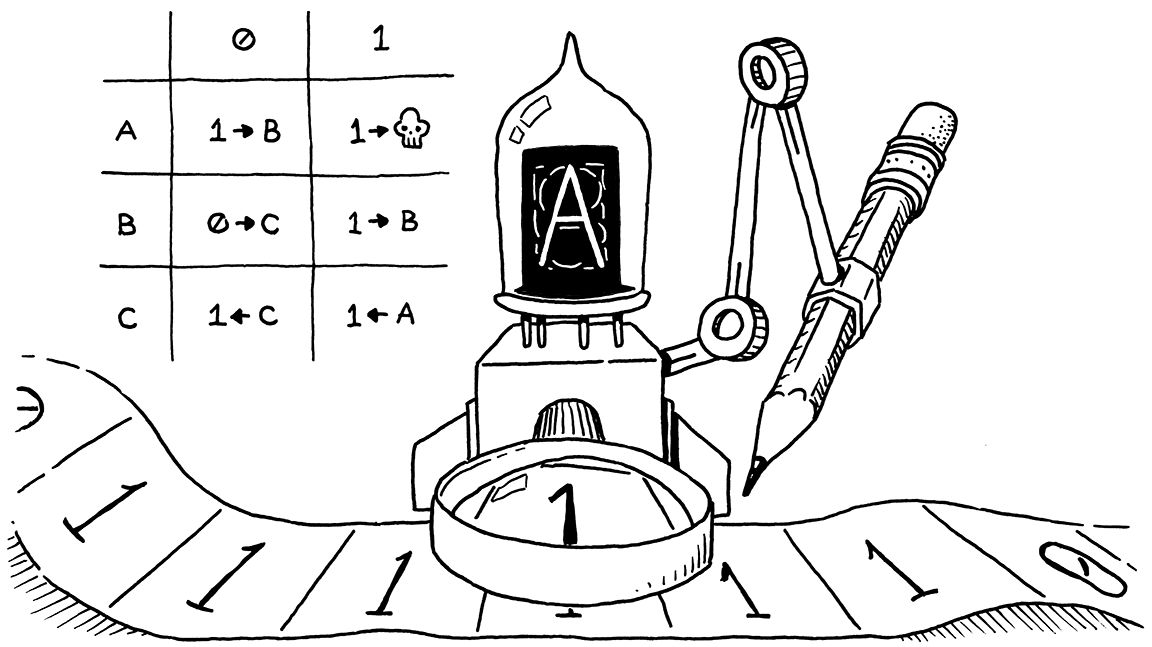
\includegraphics[width=.9\textwidth, keepaspectratio]{./pics/turing-machine-titlepage.png}
                \end{center}

                \vfill

                \par\noindent\rule{\textwidth}{0.8pt}
                \vspace*{0.6cm}
                \large
                \emph{Anno Accademico 2021-2022}

                \newpage

                \vspace*{0.5cm}
                \vfill
                \large

                Un grazie va a \emph{Matthew Butterick}, ed ai suoi preziosissimi consigli sull'uso corretto (e responsabile) della tipografia.

                https://practicaltypography.com/

        \end{center}
\end{titlepage}

